\documentclass[border=0.5cm]{standalone}
\usepackage{color}
\usepackage{bm}
\usepackage{tikz}
\usetikzlibrary{shapes,arrows,arrows.meta,fit,positioning}
\usetikzlibrary{chains,quotes}

\newcommand{\defaultwidth}{3.25cm}
\newcommand{\tseparation}{7cm}
\tikzset{
    auto, node distance = 2cm,
    stage/.style = { draw, very thick, rectangle, align=center,
        node distance = 2cm,
        text width = \defaultwidth, 
        font=\bfseries,
        rounded corners=2mm, 
        minimum width = \defaultwidth
    },
    notes/.style = { draw, very thin, rectangle, dashed, align=left,
        node distance = 1.5cm,
        text width = \defaultwidth + 1.5cm, 
        font=\footnotesize,
        minimum width = \defaultwidth + 1.5cm
    },
    arrow_text/.style = { align=left,
        pos = 0.5,
        text width = \defaultwidth, 
        font = \footnotesize,
        minimum width = \defaultwidth
    },
    point/.style = { draw, circle, fill,
        inner sep = 0.1cm,
        node contents={}
    },
    aline/.style = { very thick, minimum width = 10cm },
    arrow/.style = { ->, very thick }
}

\begin{document}
    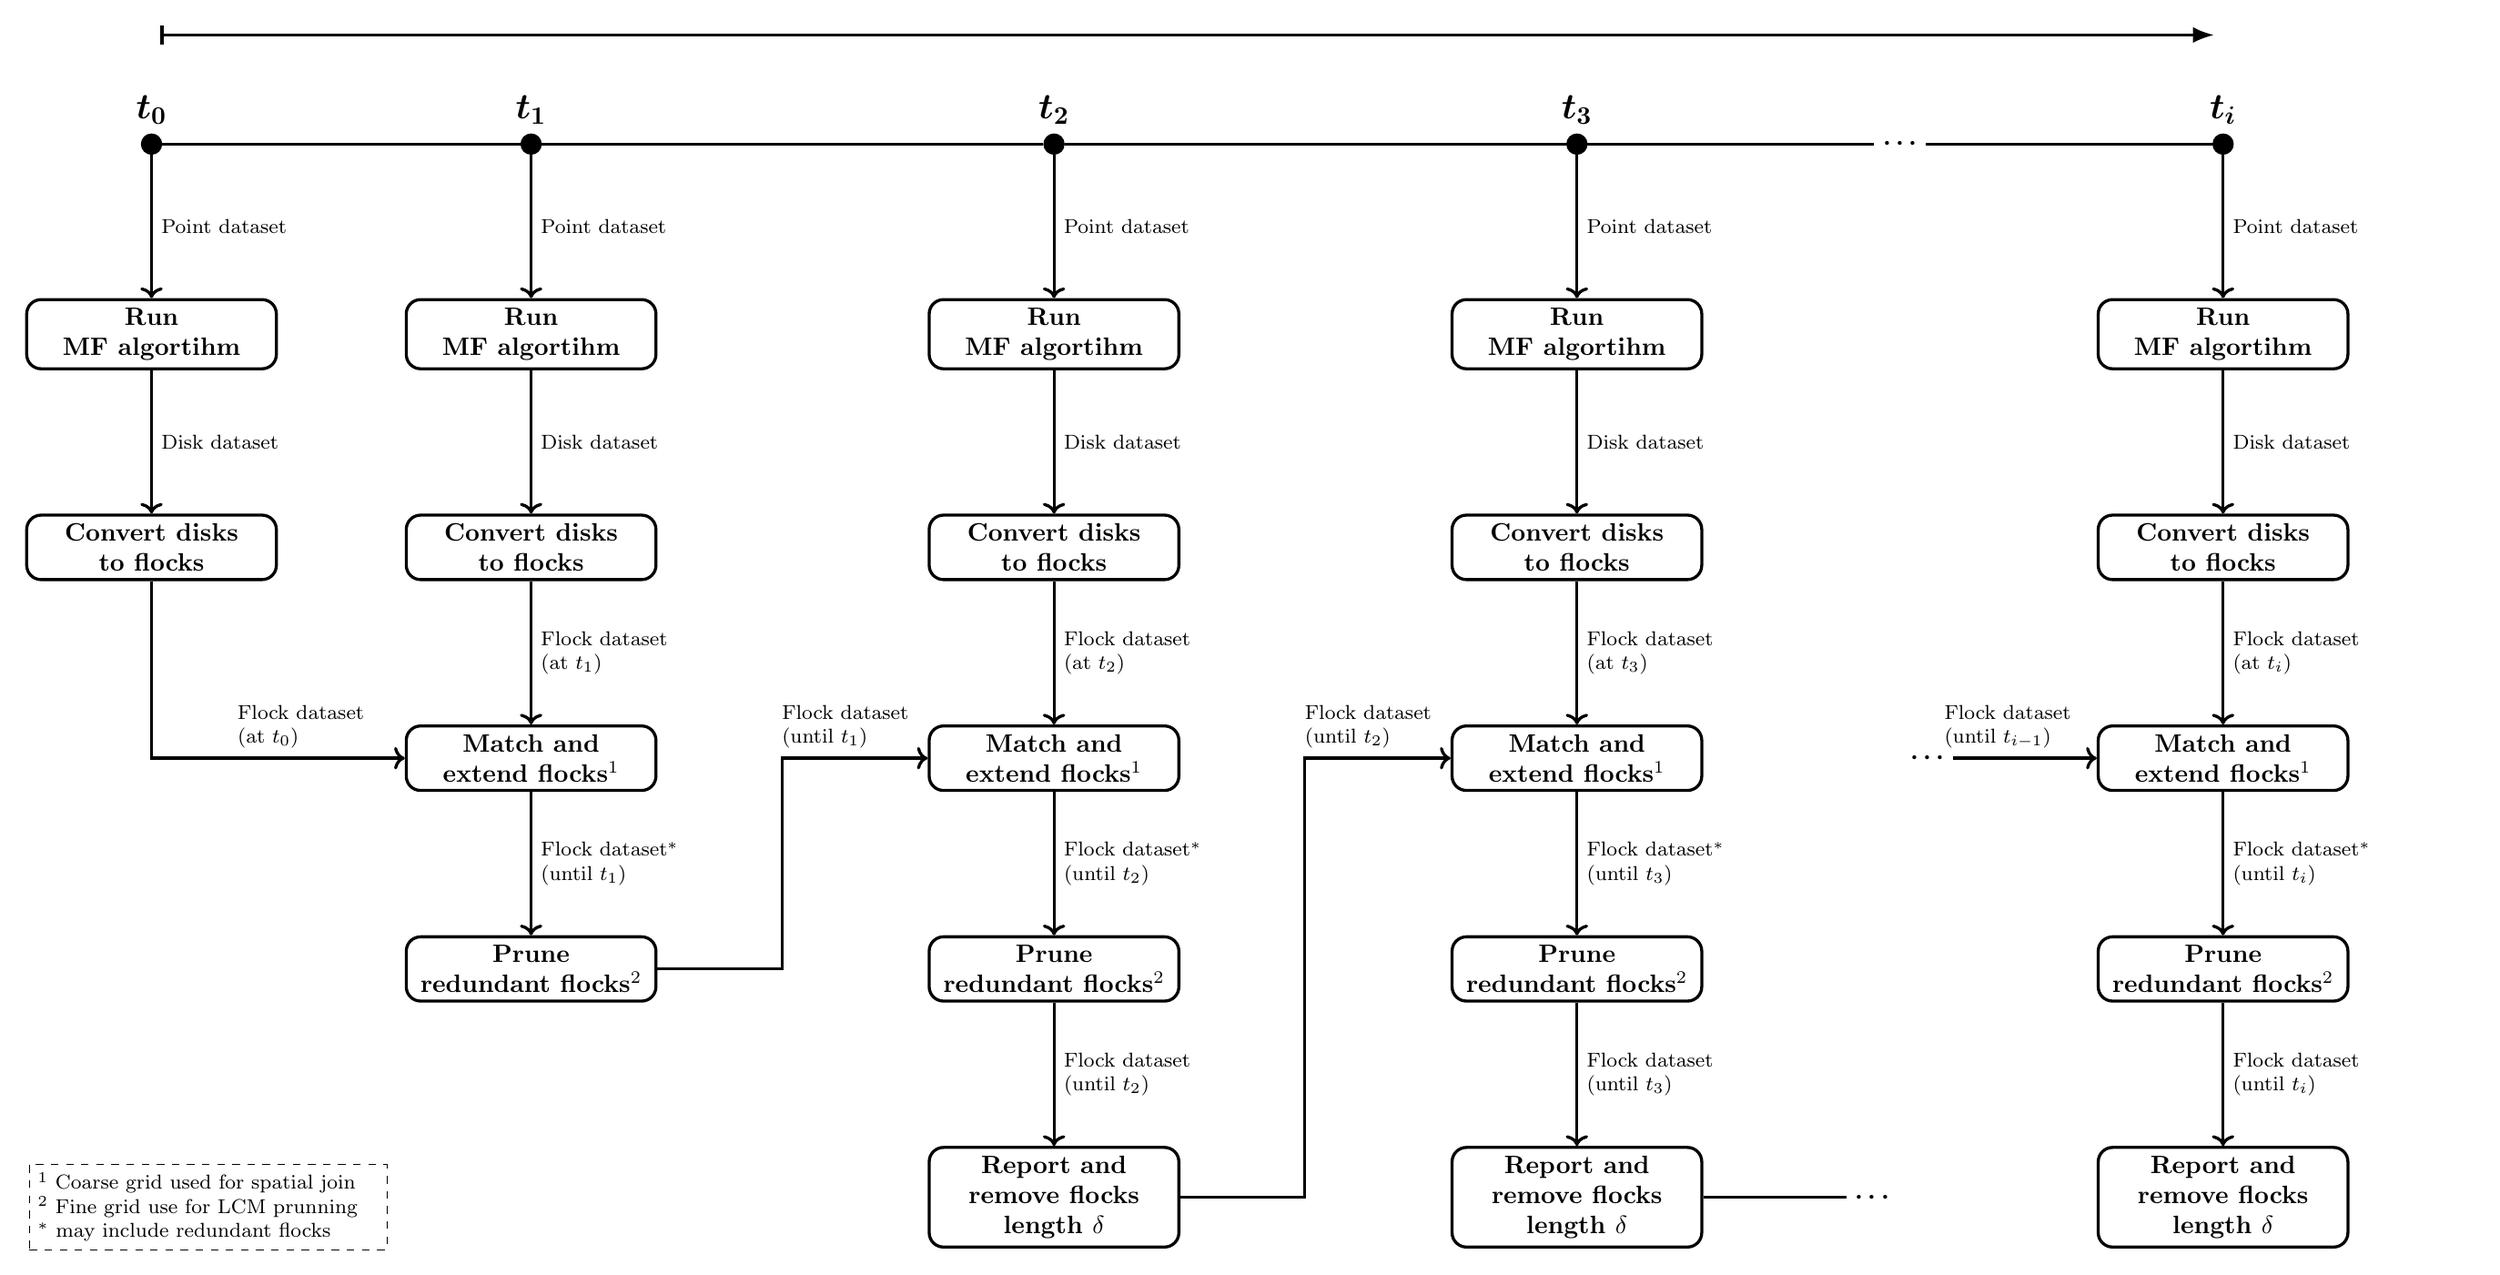
\begin{tikzpicture}
        \node (t0) at (0,0) [label=above:{\Large \bm{$t_0$}}, point];
        \node (t1) [right=5cm of t0] [label=above:{\Large \bm{$t_1$}}, point];
        \node (t2) [right=\tseparation of t1] [label=above:{\Large \bm{$t_2$}}, point];
        \node (t3) [right=\tseparation of t2] [label=above:{\Large \bm{$t_3$}}, point];
        \node (t)  [right=4cm of t3] {\bm{$\cdots$}};
        \node (ti) [right=4cm of t] [label=above:{\Large \bm{$t_i$}}, point];
        \node (a) [above = 1.25cm of t0] [node contents={}];
        \node (b) [above = 1.25cm of ti] [node contents={}];
        \path[|-Latex, draw, very thick] (a) -- (b);

        \path[aline] (t0) edge (t1);
        \path[aline] (t1) edge (t2);
        \path[aline] (t2) edge (t3);
        \path[aline] (t3) edge (t);
        \path[aline] (t)  edge (ti);
        
        % t0 branch...
        \node[stage] (t01) [below = of t0]  {Run\\ MF algortihm};
        \draw[arrow] (t0)  -- node[arrow_text] {Point dataset} (t01);
        \node[stage] (t02) [below = of t01] {Convert disks to flocks};
        \draw[arrow] (t01) -- node[arrow_text] {Disk dataset} (t02);

        % t1 branch...
        \node[stage] (t11) [below = of t1]  {Run\\ MF algortihm};
        \draw[arrow] (t1)  -- node[arrow_text] {Point dataset} (t11);
        \node[stage] (t12) [below = of t11] {Convert disks to flocks};
        \draw[arrow] (t11) -- node[arrow_text] {Disk dataset} (t12);
        \node[stage] (t13) [below = of t12] {Match and extend flocks$^1$};
        \draw[arrow] (t02) |- node[arrow_text, pos = 0.9] {Flock dataset\\ (at $t_0$)} (t13); 
        \draw[arrow] (t12) -- node[arrow_text] {Flock dataset\\ (at $t_1$)} (t13);
        \node[stage] (t14) [below = of t13] {Prune\\ redundant flocks$^2$};
        \draw[arrow] (t13) -- node[arrow_text] {Flock dataset$^*$\\ (until $t_1$)} (t14);
        
        % t2 branch...
        \node[stage] (t21) [below = of t2]  {Run\\ MF algortihm};
        \draw[arrow] (t2)  -- node[arrow_text] {Point dataset} (t21);
        \node[stage] (t22) [below = of t21] {Convert disks to flocks};
        \draw[arrow] (t21) -- node[arrow_text] {Disk dataset} (t22);
        \node[stage] (t23) [below = of t22] {Match and extend flocks$^1$};
        \draw[arrow] (t14) -|  ++(3.5,2) |- node[arrow_text, pos = 0.9] {Flock dataset\\ (until $t_1$)} (t23); 
        \draw[arrow] (t22) -- node[arrow_text] {Flock dataset\\ (at $t_2$)} (t23);
        \node[stage] (t24) [below = of t23] {Prune\\ redundant flocks$^2$};
        \draw[arrow] (t23) -- node[arrow_text] {Flock dataset$^*$\\ (until $t_2$)} (t24);
        \node[stage] (t25) [below = of t24] {Report and remove flocks length $\delta$};
        \draw[arrow] (t24) -- node[arrow_text] {Flock dataset\\ (until $t_2$)} (t25);
        
        % t3 branch...
        \node[stage] (t31) [below = of t3]  {Run\\ MF algortihm};
        \draw[arrow] (t3)  -- node[arrow_text] {Point dataset} (t31);
        \node[stage] (t32) [below = of t31] {Convert disks to flocks};
        \draw[arrow] (t31) -- node[arrow_text] {Disk dataset} (t32);
        \node[stage] (t33) [below = of t32] {Match and extend flocks$^1$};
        \draw[arrow] (t25) -|  ++(3.5,2) |- node[arrow_text, pos = 0.9] {Flock dataset\\ (until $t_2$)} (t33); 
        \draw[arrow] (t32) -- node[arrow_text] {Flock dataset\\ (at $t_3$)} (t33);
        \node[stage] (t34) [below = of t33] {Prune\\ redundant flocks$^2$};
        \draw[arrow] (t33) -- node[arrow_text] {Flock dataset$^*$\\ (until $t_3$)} (t34);
        \node[stage] (t35) [below = of t34] {Report and remove flocks length $\delta$};
        \draw[arrow] (t34) -- node[arrow_text] {Flock dataset\\ (until $t_3$)} (t35);

        % ...
        \node (f1) [right=2cm of t35] {\bm{$\cdots$}};
        \path[aline] (t35) edge (f1);
        
        % ti branch...
        \node[stage] (ti1) [below = of ti]  {Run\\ MF algortihm};
        \draw[arrow] (ti)  -- node[arrow_text] {Point dataset} (ti1);
        \node[stage] (ti2) [below = of ti1] {Convert disks to flocks};
        \draw[arrow] (ti1) -- node[arrow_text] {Disk dataset} (ti2);
        \node[stage] (ti3) [below = of ti2] {Match and extend flocks$^1$};
        \draw[arrow] (ti2) -- node[arrow_text] {Flock dataset\\ (at $t_i$)} (ti3);
        \node[stage] (ti4) [below = of ti3] {Prune\\ redundant flocks$^2$};
        \draw[arrow] (ti3) -- node[arrow_text] {Flock dataset$^*$\\ (until $t_i$)} (ti4);
        \node[stage] (ti5) [below = of ti4] {Report and remove flocks length $\delta$};
        \draw[arrow] (ti4) -- node[arrow_text] {Flock dataset\\ (until $t_i$)} (ti5);

        % ...
        \node (f2) [left=2cm of ti3] {\bm{$\cdots$}};
        \draw[arrow] (f2) -- node[arrow_text, pos=0.75] {Flock dataset\\ (until $t_{i-1}$)} (ti3);

        % Notes...
        \node[notes] (n) [below left = 2.25 and 0.25 of t14] {
            $^1$ Coarse grid used for spatial join\\ 
            $^2$ Fine grid use for LCM prunning\\ 
            $^*$ may include redundant flocks
        }; 
        
    \end{tikzpicture}
\end{document}
